\section{実験目的}
本プロジェクトでは、雑多な環境下においてロボットの最大直進速度で追従できる人追従システムの
開発を目的としている。これに伴った実験の目的は、雑多な環境下での人追従の制度とロボットの
最大直進速度での人追従性能の2つの検証をすることである。以上のことから、追従実験と最大
追従速度実験により、開発した人追従システムの性能を検証する。

\section{実験方法}
実験では、雑多な環境を作成し追従実験と最大追従速度実験をする。
実験中は、人は追従対象の1人のみとする。\\ \indent
要求仕様(2)を検証するため、追従実験では直線経路、曲線経路、直角経路をそれぞれ10回実験し、
成功率を算出する。追従の成功率が平均90\%以上であった場合に要求仕様(2)を満たしたものとする。
また、要求仕様(3)を検証するため、10[m]以上の直線経路にて最大追従速度実験をする。
0.1[m/s]から、0.1ずつ速度を上昇させ、追従できなくなる速度の直前を最大追従速度とする。
Turtlebot3 Big Wheelの最大直進速度が0.5[m/s]であるため、開発した人追従システムの
最大追従速度が0.5[m/s]であった場合に要求仕様(3)は満たされる。
以上の実験は、2D-LiDARのデータを用いた実験であるため、要求仕様(2)、(3)が満たされたら、
要求仕様(1)も満たされたものとする。

\subsection{実験機材}
\begin{figure*}[h]
  \begin{center}
  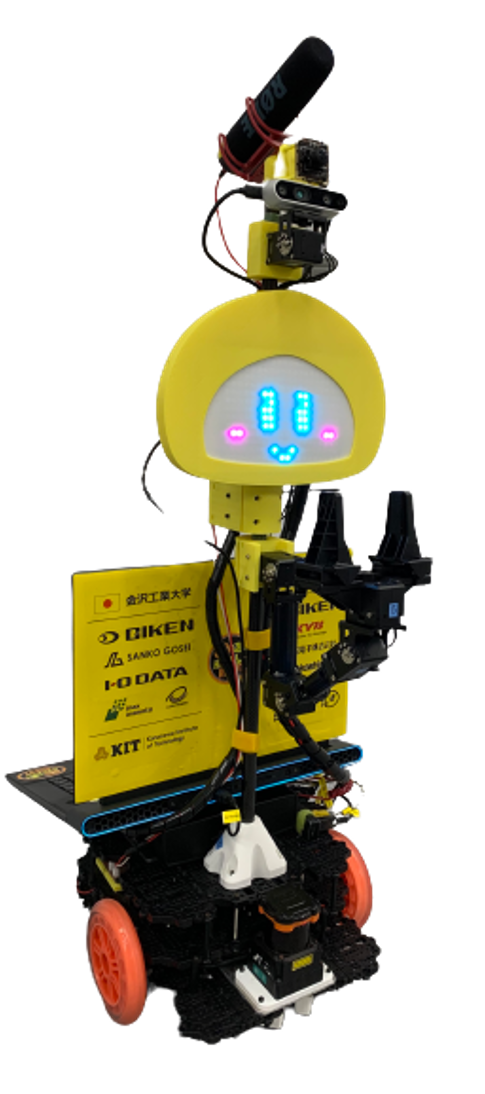
\includegraphics[width=30mm,clip]{figure/Happy_Edu.png}
  \caption{Happy Edu}
  \label{Happy Edu}
  \end{center}
\end{figure*}

\begin{table}[h]
  \begin{center}
    \caption{{Happy Edu specifications}\label{Happy Edu specifications}}
    \scalebox{0.8}[0.9]{
      \begin{tabular}{c|c|c} \hline
        Type of equipment & Product name & Specifications \\ \hline
        Robot base & Turtlebot3 Big Wheel & 
        \begin{tabular}{c}
        Maximum straight speed: 0.6[m/s]\\
        Maximum rotation speed: 3.14[rad/s]\\
        Maximum payload: 30[kg]\\
        Size(length x width x height): 281mm x 306mm x 170.30 [mm]
        \end{tabular} \\ \hline
        Robot laptop & ASUS ROG Strix G16 &  
        \begin{tabular}{c}
        CPU: Corei7 13650HX\\
        GPU: GeForce RTX4070 8GB\\
        Weight: 2.5 [kg]\\
        Size: 26.4 x 35.4 x 2.26 [cm]\\
        \end{tabular} \\ \hline
        2D-LiDAR & UTM-30LX & 
        \begin{tabular}{c}
        Maximum detection distance: 60 [m]\\
        Scan range: 270 [deg]\\
        Angle resolution energy: 0.25 [deg]\\
        Scan time: 25 [ms]
        Weight: 210 [g]
        \end{tabular} \\ \hline
      \end{tabular}
    }
  \end{center}
\end{table}

\subsection{実験環境}

\subsection{追従実験}
\begin{figure*}[h]
  \begin{center}
  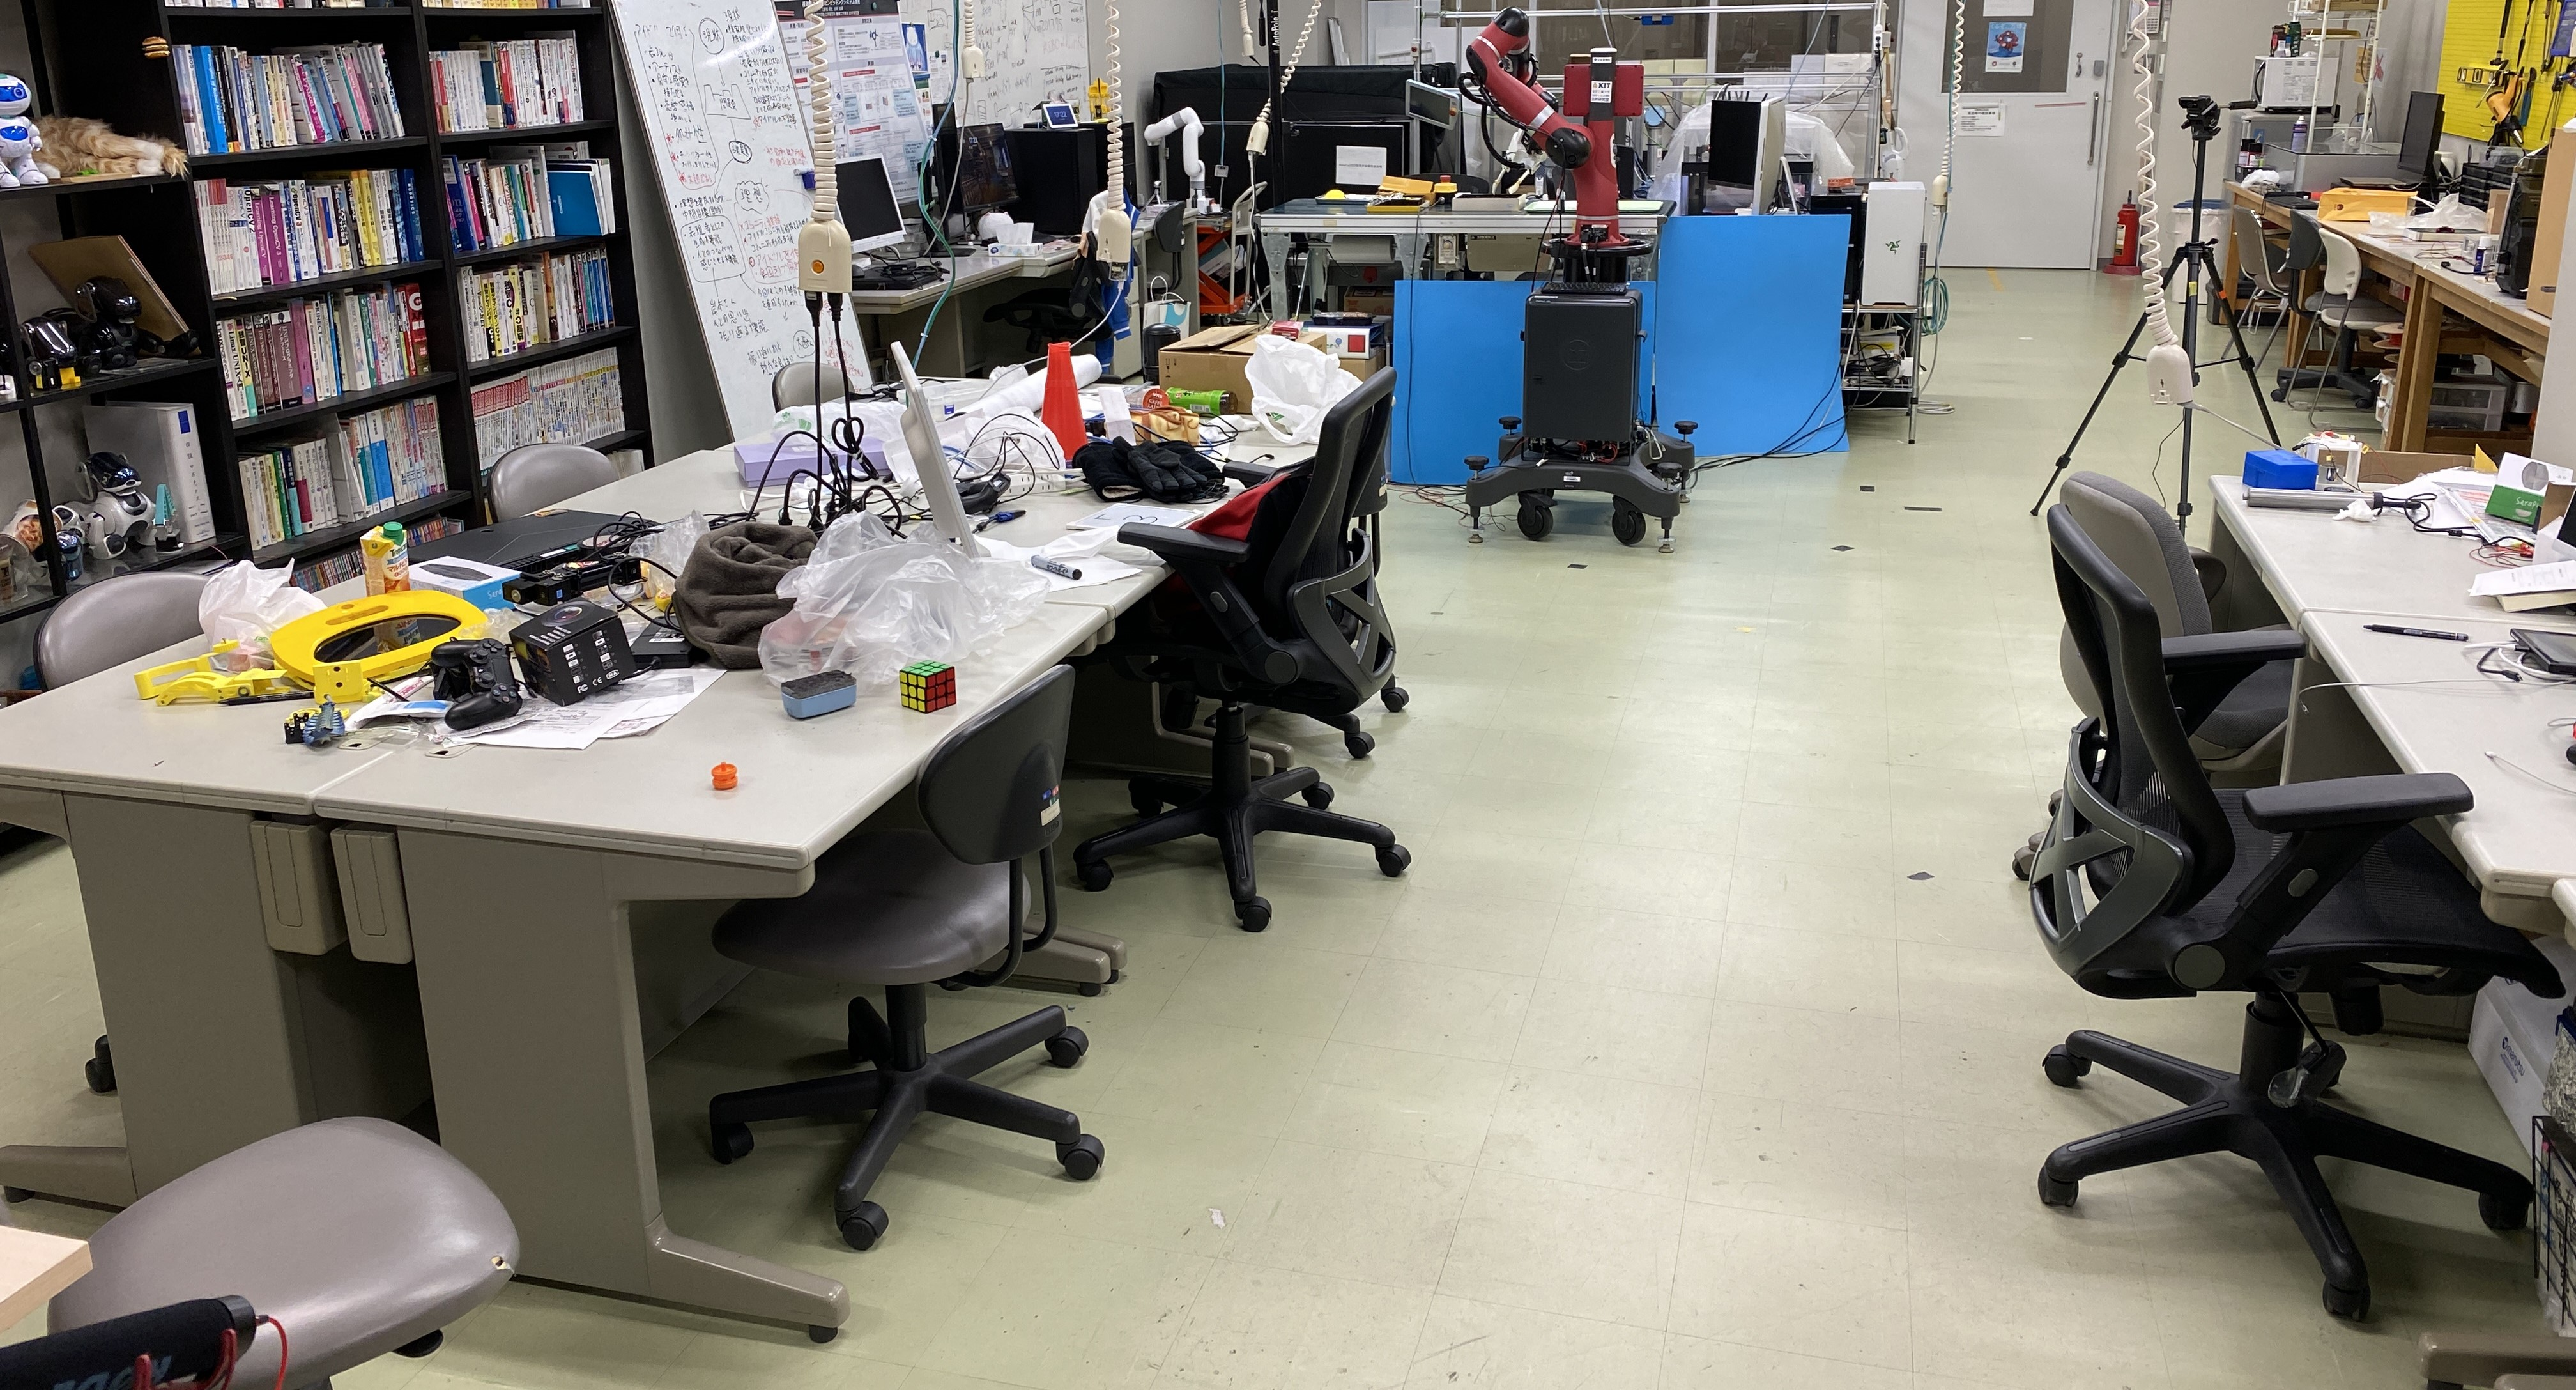
\includegraphics[width=100mm,clip]{figure/experimental_env1.JPG}
  \caption{Image of tracking experiment environment (FMT Laboratory Room 206)}
  \label{Image of tracking experiment environment (FMT Laboratory Room 206)}
  \end{center}
\end{figure*}

\begin{figure*}[h]
  \begin{center}
  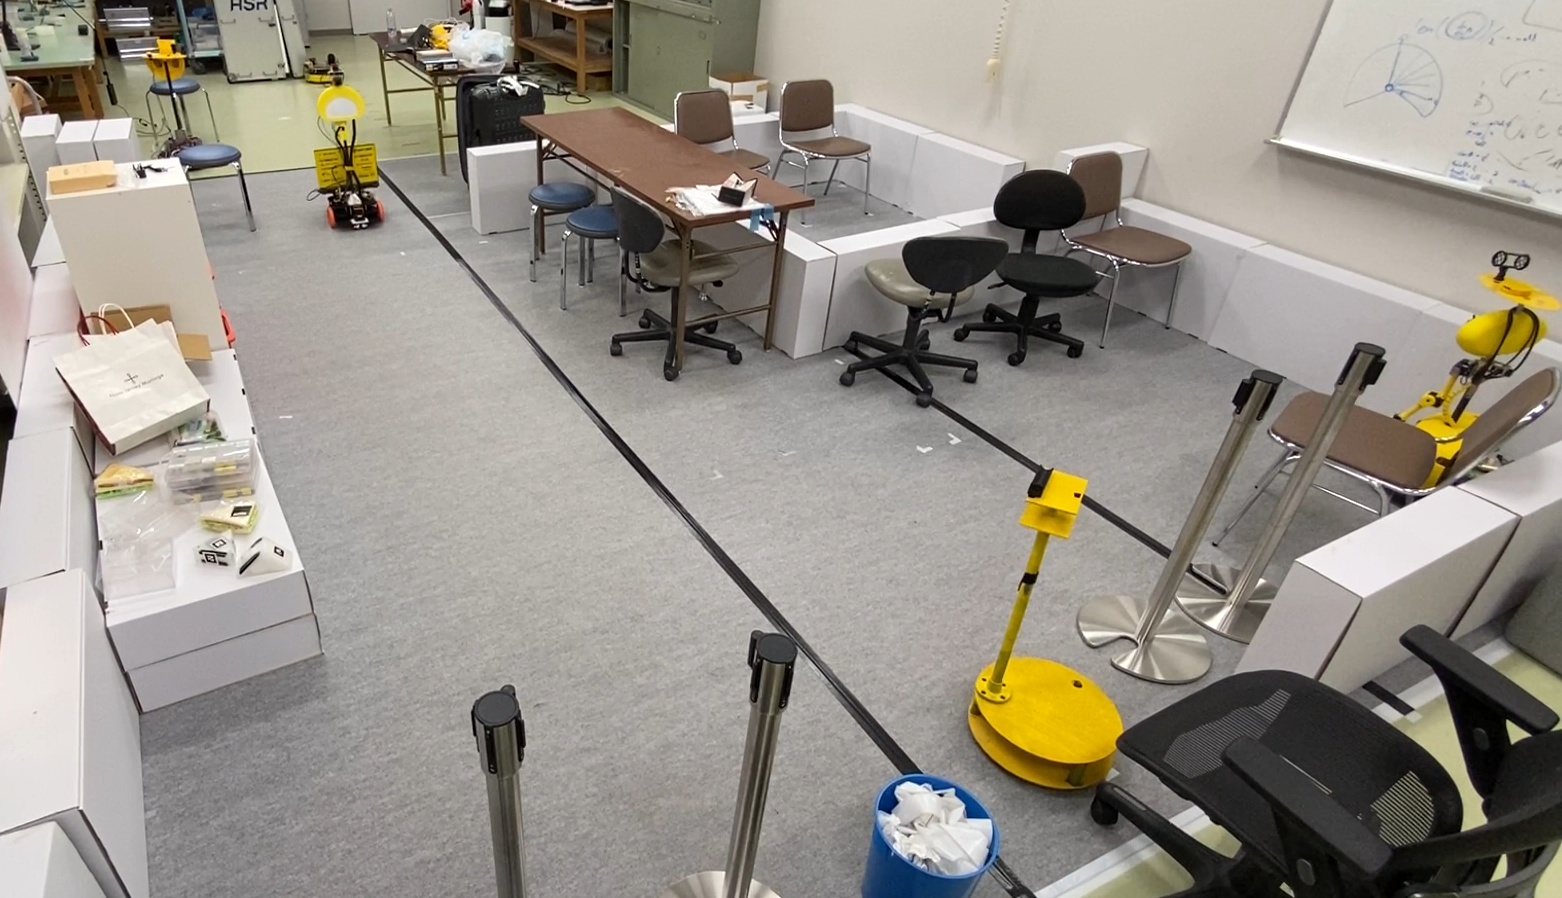
\includegraphics[width=100mm,clip]{figure/experimental_env2.png}
  \caption{Image of tracking experiment environment (FMT Laboratory Room 326)}
  \label{Image of tracking experiment environment (FMT Laboratory Room 326)}
  \end{center}
\end{figure*}

\subsection{最大追従速度実験}
\begin{figure*}[h]
  \begin{center}
  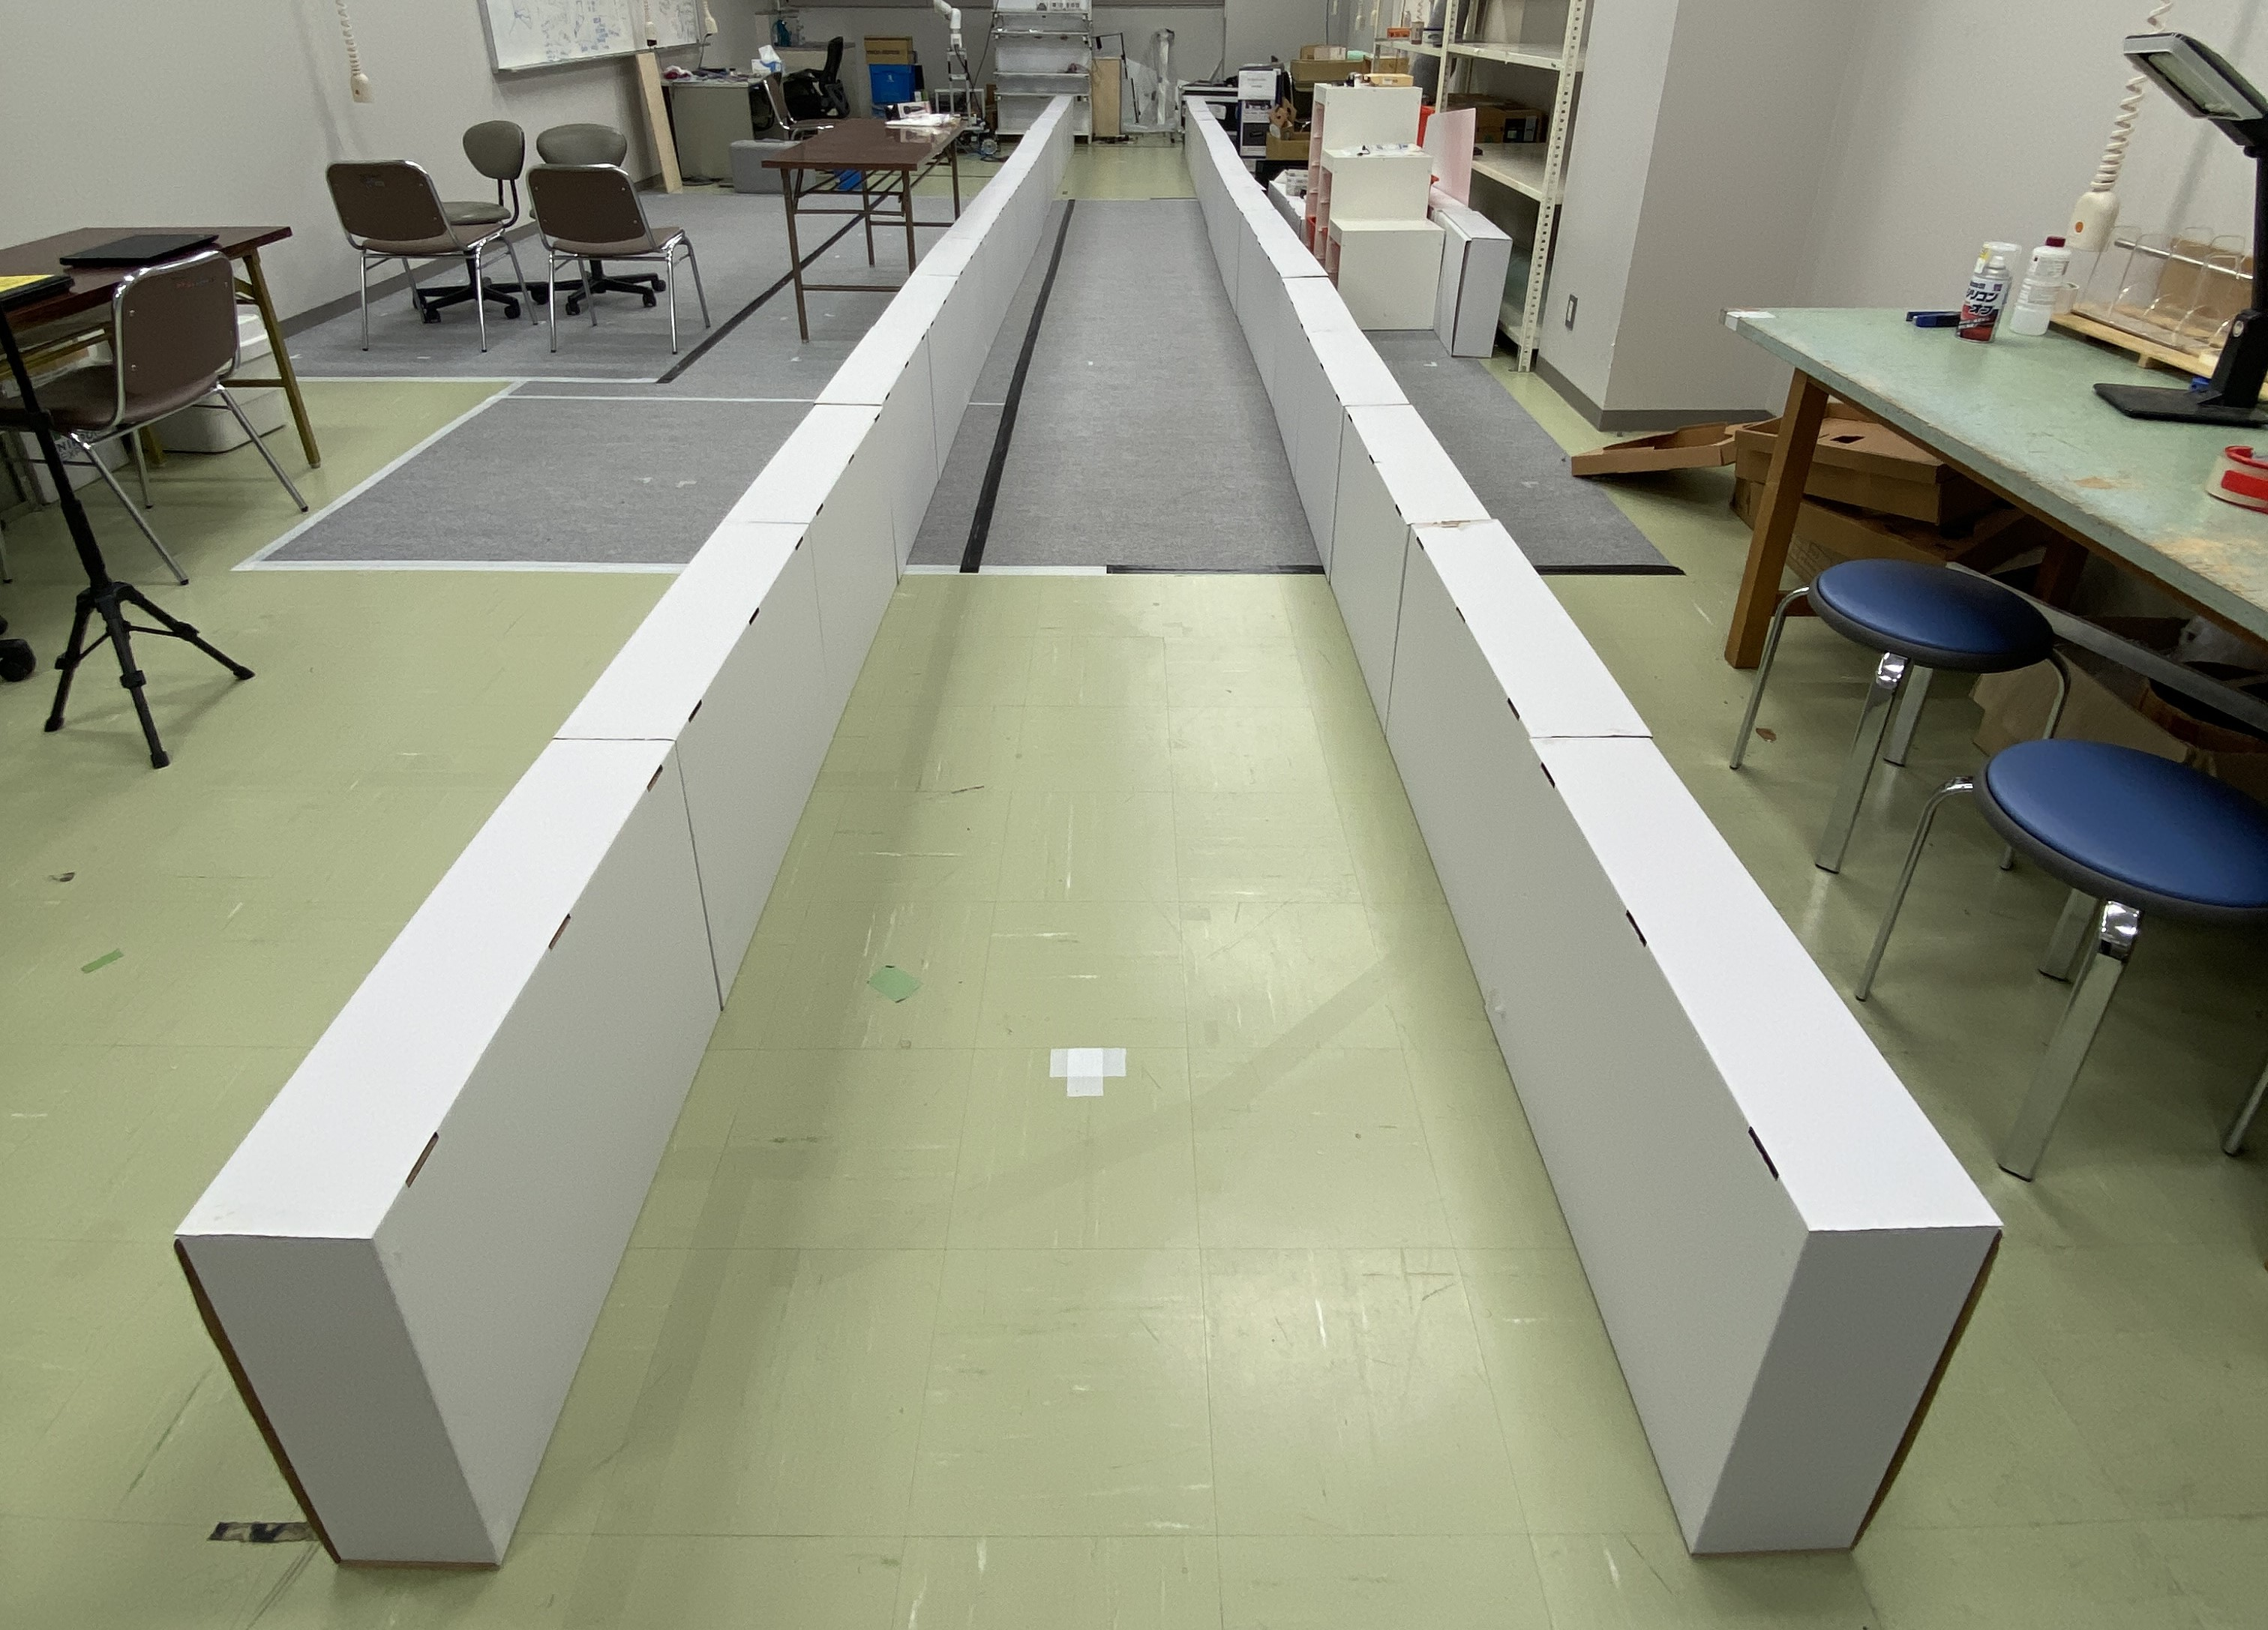
\includegraphics[width=100mm, angle=-90, clip]{figure/experimental_env3.JPG}
  \caption{Maximum tracking speed experiment environment image (FMT Laboratory Room 326)}
  \label{Maximum tracking speed experiment environment image (FMT Laboratory Room 326)}
  \end{center}
\end{figure*}

\begin{figure*}[h]
  \begin{center}
  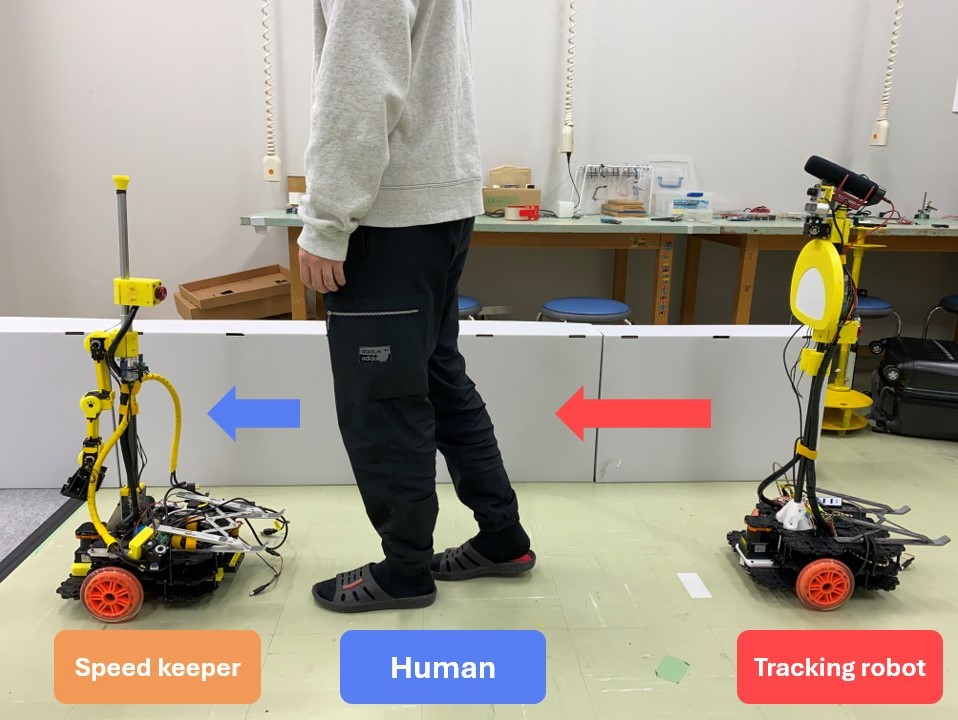
\includegraphics[width=100mm,clip]{figure/max_experiment_image.JPG}
  \caption{Image of maximum tracking speed experiment}
  \label{Image of maximum tracking speed experiment}
  \end{center}
\end{figure*}

\section{実験結果}
\subsection{追従実験}
\begin{figure*}[h]
  \begin{center}
  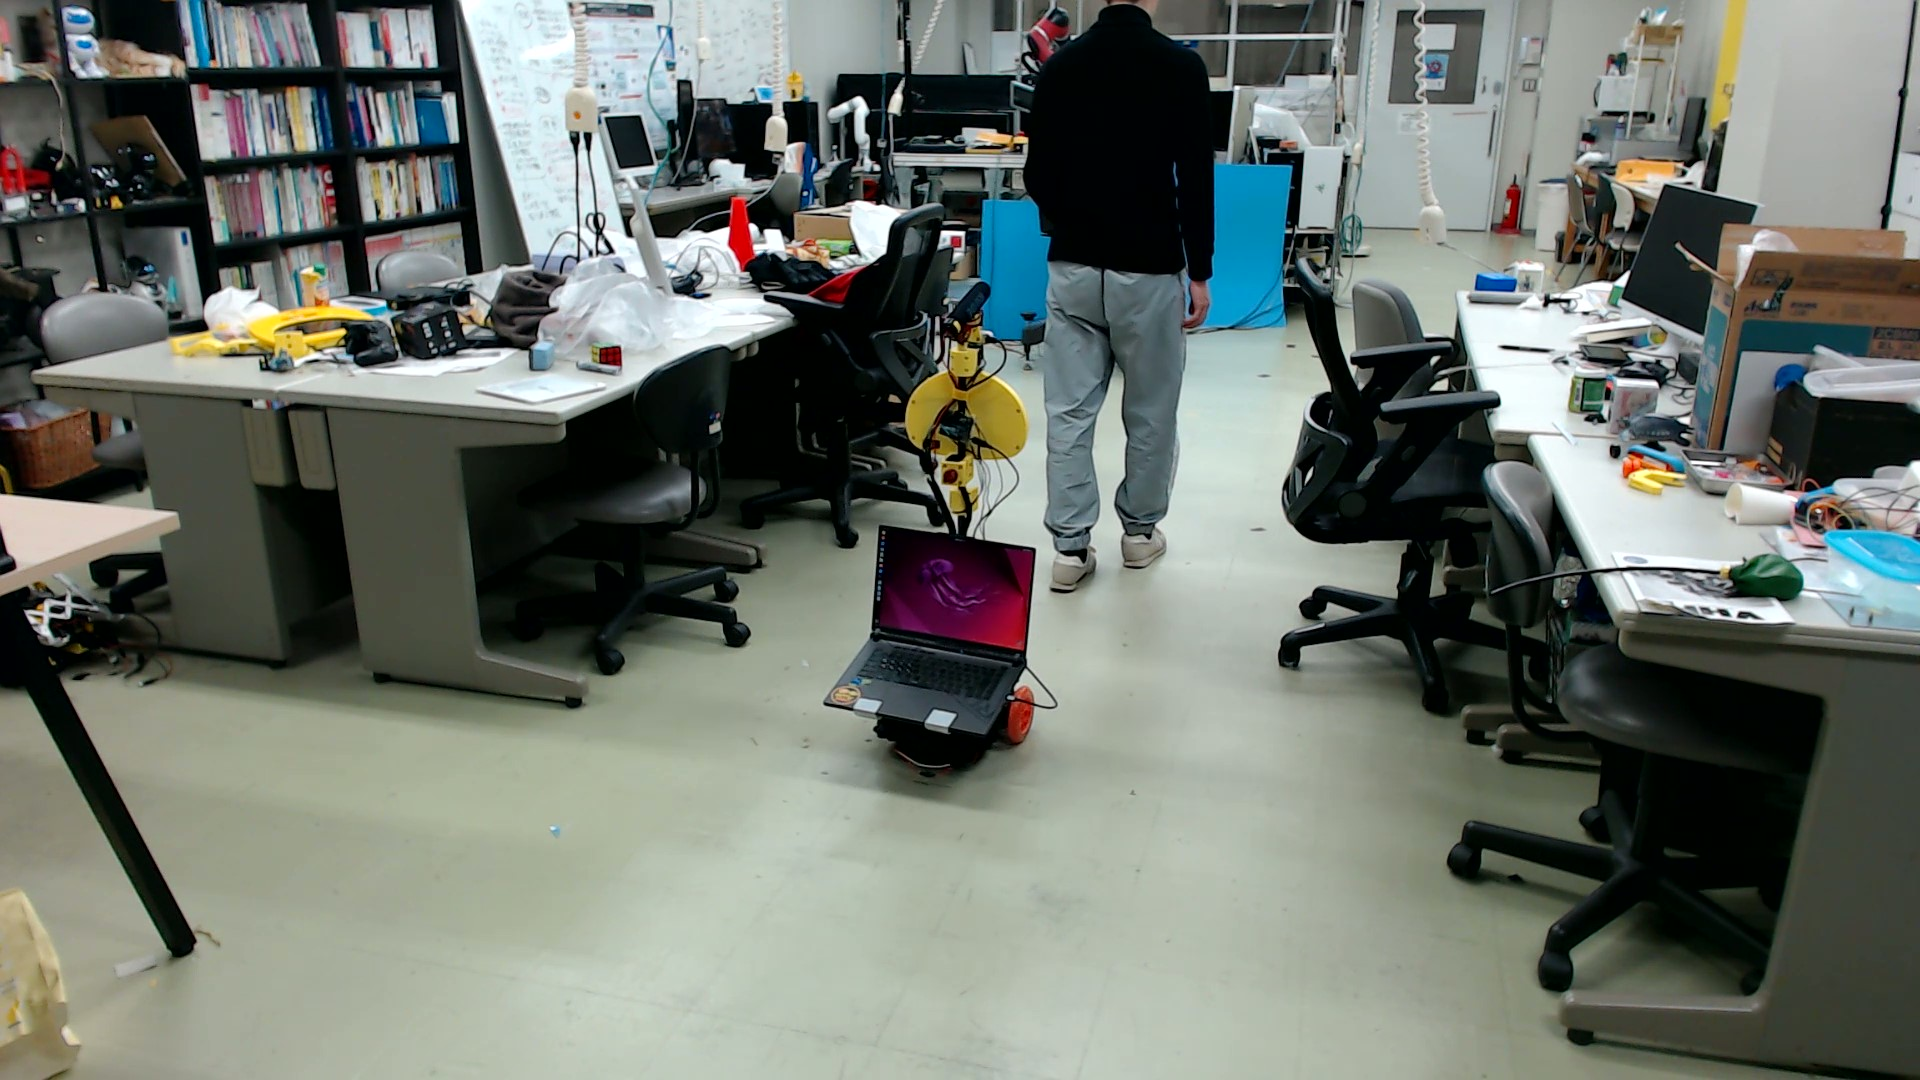
\includegraphics[width=100mm,clip]{figure/Tracking-experiment-Real-view.jpg}
  \caption{Tracking experiment (Real view)}
  \label{Tracking experiment (Real view)}
  \end{center}
\end{figure*}

\begin{figure*}[h]
  \begin{center}
  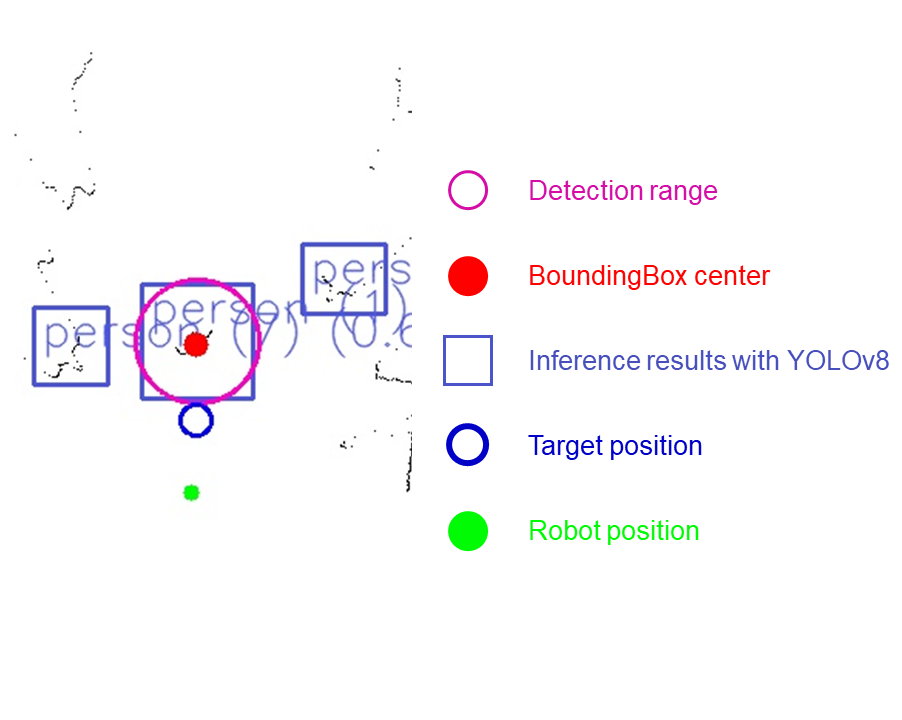
\includegraphics[width=170mm,clip]{figure/Tracking-experiment-Internal-view.png}
  \caption{Tracking experiment (Internal view)}
  \label{Tracking experiment (Internal view)}
  \end{center}
\end{figure*}

\begin{table}[h]
    \begin{center}
      \caption{{Success rate of traking in each road}\label{Success rate of traking in each road}}
      \scalebox{1.2}[1.0]{
        \begin{tabular}{c|r} \hline
          Road & Success rate [\%] \\ \hline
          Straight road & 100 \\
          Curved road & 100 \\
          Right angle road & 100 \\ \hline
        \end{tabular}
      }
    \end{center}
\end{table}

直線経路、曲線経路、直角経路、最大追従速度の実験結果をFig. \ref{Result}に示す。
追従実験では、直線経路と直角経路がそれぞれ10回中10回成功した。曲線経路では、10回中9回成功した。

\subsection{最大追従速度実験}

\begin{table}[h]
  \begin{center}
    \caption{{Maximum tracking speed experimental result}\label{Maximum tracking speed experimental result}}
    \scalebox{1.0}[0.9]{
      \begin{tabular}{c|r} \hline
        Tracking speed [m/s] & Travel distance tracked [m] \\ \hline
        0.1 & 11.73 \\
        0.2 & 11.31 \\
        0.3 & 11.58 \\
        0.4 & 11.53 \\
        0.5 & 11.48 \\
        0.6 & 6.231 \\ \hline
      \end{tabular}
    }
  \end{center}
\end{table}

\begin{figure*}[h]
  \begin{center}
  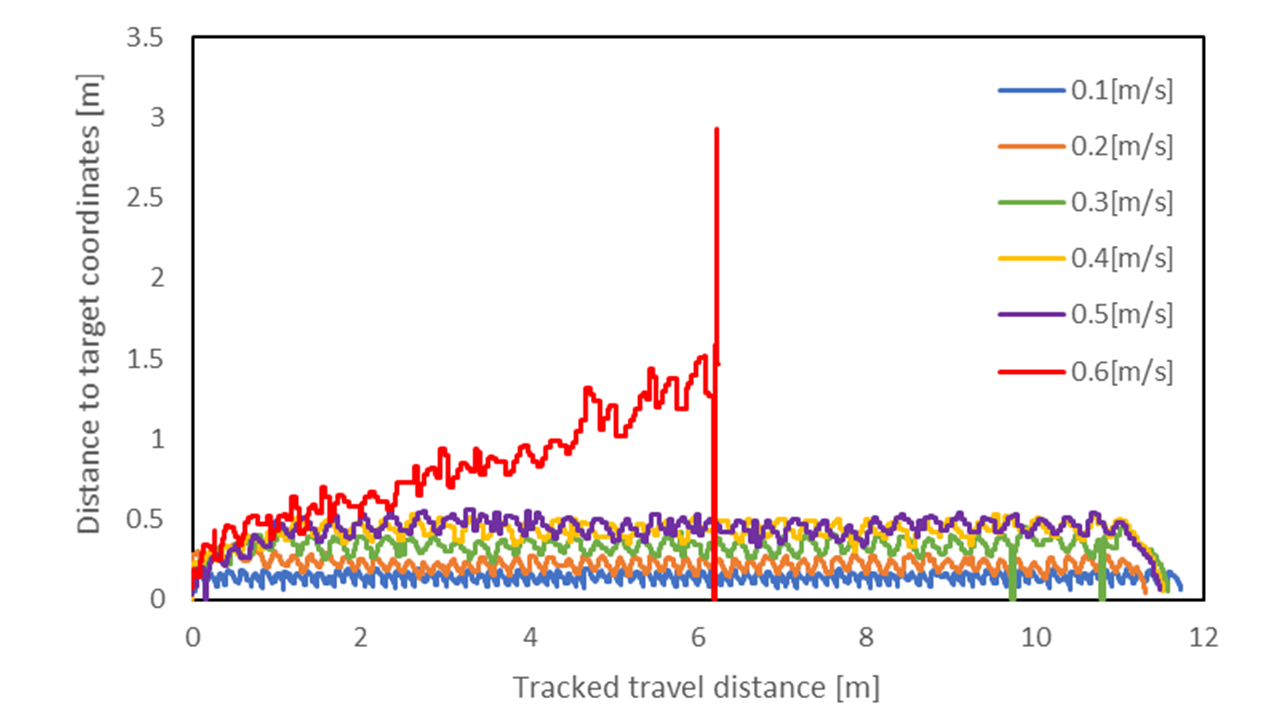
\includegraphics[width=150mm,clip]{figure/Maximum-tracking-speed-experimental-result.png}
  \caption{Tracking speed graph}
  \label{Tracking speed graph}
  \end{center}
\end{figure*}

最大追従実験では、0.5[m/s]が最大追従速度となった。0.6[m/s]で3回実験したが、追従は確認されなかった。

\section{考察}
実験結果から直線経路と直角経路では、雑多な環境において一度も止まらず安定した挙動で要求仕様を
満たすことができた。しかし、曲線経路では一度だけ停止した。曲線経路で停止した原因は、ロボット用ノートPCのバッテリー低下だと考えられる。ロボットが停止しなかった場合のROS2 bagでは、システム全体の通信が平均10[Hz]以上で安定しているのに対し、曲線経路で停止したときは、平均4.9[Hz]であった。実験が成功しているROS2 bagでは、通信速度の低下は確認されず、ノートPCのバッテリーが10\%以下であったのは、曲線経路で停止した場合のみであった。